See appendix \ref{cudaAppendix} for a review of the Cuda parallel processing framework.
\subsection{Cuda Implementation: Iterative}
The iterative form of the FFT algorithm is well suited for execution on a GPU. The strategy will be to treat each executing thread as single entry in the array. That is, each thread is responsible for computing the FFT value of the array location given by its global index. 

Three kernels are used to perform this task: \texttt{bit\_reverse\_kernel()}, \texttt{fft\_kernel\_shared()}, and \texttt{fft\_kernel\_finish()}. The sequence of execution in the FFT computation goes like this:
\begin{itemize}
    \item Load input data from CPU to GPU
    \item call \texttt{bit\_reverse\_kernel()} to perform array index bit-reversal in global memory
    \item call \texttt{fft\_kernel\_shared()} to perform the partial FFT using shared memory
    \item loop over \texttt{fft\_kernel\_finish()} to finish the FFT in global memory
    \item Retrieve data from GPU memory to CPU
\end{itemize}

This implementation computes all the partial FFTs in shared memory. That is, due to the thread block-size restriction of 1024 threads, this approach was not able to continue with shared memory after the FFT 1024-point FFT has been performed. The limitations were that thread synchronization during kernel execution is limited to the threads within a block, and that threads from neighboring blocks cannot access each other's shared memory.

After the shared memory computation has finished, the CPU code loops over the \texttt{fft\_kernel\_finish()} kernel, which performs one iteration of the iterative FFT loop. This was thought to be necessary so that global device synchronization could be achieved. Otherwise, since the FFT algorithm now needs to reach beyond the limits of thread-block size to continue ($m/2 > 512$), there is the potential to introduce a race condition as each block proceeds out of sync with the others. 

We implemented only the iterative FFT in cuda due to the natural programming style of GPU computations: GPUs are not ideally suited for recursive tasks. However, it is now possible to launch new grids of threads from an executing grid, where previously new grids (kernels) could only be launched from the CPU. This technique is know as Dynamic Parallelism, and enables recursive programming on the GPU. We did not explore this option, but felt it is important to mention.

\subsection{Cuda Analysis}
The performance of our cuda FFT is shown in figure \ref{cudaRuntimes}. This graph includes the numpy FFT, our cuda impementation, and the Nvidia CUFFT library function. For both cuda algorithms, full times and ``inner" times are plotted. The full time includes data transfer from CPU to GPU and back, and the inner time measures only the actual FFT computation. The total time does not include a CUDA device initialization, which can take hundreds of milliseconds.

Several interesting features are visible on the graph. Most obvious is that the CUFFT total time is significantly larger than any other of the displayed algorithms. This is due in part to the CPU/GPU memory transfer, but primarily it comes from the requirement to compute an FFT plan, which optimizes the run configuration when executing an FFT with CUFFT. For our cuda implementation, a fairly consistent amount of additional time is required for the data transfer, though the difference shrinks as $N$ increases. This is because the data transfer time is only $\mathcal{O}(N)$, while the thread saturated cuda run time is $\mathcal{O}(N\log N)$. For $N<1024$, the sequential numpy FFT outperforms either cuda implementation. A large spike in CUFFT is seen at $N=2^{12}$, which is expected based on the Nvidia published CUFFT performance tests. Between 1024 and $2^{15}$, our cuda implementation grows very slowly. After $2^{15}$, however, the cuda codes start to grow with the same slope as the numpy FFT. This makes sense: the GPUs available on Stampede are Nvidia K20m cards, which have can run a maximum of 26624 concurrent threads. The number $26624 \approx 2^{14.7}$, so the turning point in the cuda performance curve at about $2^{15}$ is expected by Brent's Scheduling Principle. Even for large values of $N$, however, our implementation performs about 10 times faster than numpy, and the built-in CUFFT is about 100x faster.

\begin{figure}
    \centering
    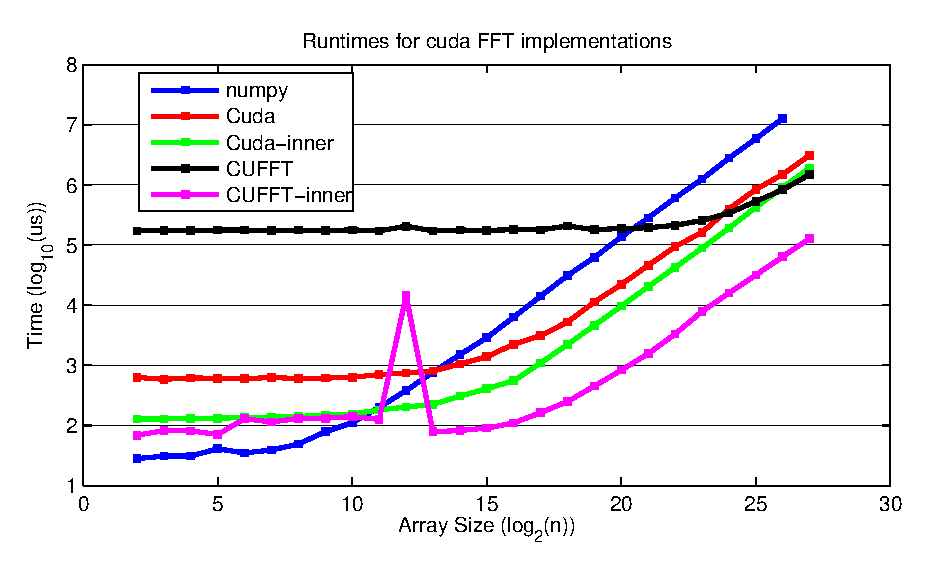
\includegraphics[scale=0.75]{img/cudaRuntimes.eps}
    \caption{Comparison of cuda FFT runtimes.}
    \label{cudaRuntimes}
\end{figure}